\chapter{Temperature gradients determination}
\label{ch:temperature_corbino}

Up to this point we have described how we measured the thermopower and conductance of the system, we also introduced the theory to describe them and the effects we aim to exploit, we shall use in the next section to model the system. From this modeling we will obtain a temperature gradient $\Delta T$, responsible of the behavior of the thermopower. So we need a way to measure the electronic system temperature, here we introduce method to do so, which is of main importance to the objectives of this thesis.

The first type of measurement one could think of is to include somehow a set of  \textcolor{azulGris}{\textbf{resistive sensors}}, thermally attached to the devices. The advantage being that they are well developed and in common use in cryogenic technologies. But, they are integrating systems, the measurement is through thermal contact so, the actual temperature measurement have to be done having several resistive sensors attached to different positions (inner outer ring) of our Corbinos, i.e. 8 sensors, 16 or 32 cables (if 4 point probing is used), meaning a complete rewiring of the probes. The actual measurement would not be of the electronic system, but an approximated value given by the crystal. 
Also, a very good electric isolation had to be obtained, otherwise the thermopower measurement would be compromise. 
The sensors should have to be glued to the devices, even with the best approach would include tensions to the crystal, resulting in a modified thermopower profile.
Because all of this, this type of arrangement was discarded.

\begin{figure}
    \centering
    \includegraphics[width = 1\textwidth]%
        {figures/temperature_corbino/probe-diagram.png}
    \caption{Dry cryoprobe images. \textit{Top left:} note the position of the temperature sensor. This sensor is the one mentioned over the thesis. Samples are mounted from below, as seen in the \textit{top right} images. Other details fo the cryoprobe can be seen in the bottom images, particularly the $^3$He heat exchange, the $^4$He pick-up line, between others.}
\end{figure}

We could also think to produce an absolute temperature measurement setup based on \textcolor{azulGris}{\textbf{Johnson noise thermometry}} \cite{Johnson1928, nyquist1928,webb1973noise,qu2019johnson}. 
In our case this would mean to set some way to thermally attach our Corbinos to such measurement system. 
It would be an approximate measuring setup, measuring each Corbino ring, approximating $\Delta T$ as a temperature difference between them. 
This type of measurement would imply to produce the measurement cryo-circuits, and probabbly would need some kind of switching system to detach its electrical connections during the thermopower and conductance measurements, not an easy task. 
This kind of measurement is absolute and reliable, but its technology and components were not available in our systems. 
Once again, given the problems described we aimed for a different approach.

From Kobayakawa, et. al \cite{kobayakawa2013diffusion} we have another temperature determination option, but implies to use also their RF measurement configuration, we could not use our heater approach.

\textcolor{azulGris}{\textbf{Temperature by conductance measurement:\\}}
Finally, since the conductance response is dependent on the temperature of the electronic system one could think of using it as temperature sensor. This is what works by Chickering et al. \cite{chickering2010thermopower}, Liu et al. \cite{Liu2018} and Endo et al.\cite{endo2019spatial} have used. They measure the thermal conductance in a Hall bar configuration to obtain a temperature for the system. 
In these cases they infer such temperature by equalizing the temperature of the system to the one of an included heater. 


We make use of such idea and take advantage of the conductance change for different powers and base temperatures, from which we are able to set a temperature gradient function, dependent of the power applied and the base temperature of the system. This approach avoids the need to include a glued sensor, for example, which would introduce problems such tensions in the crystal, extra thermal impedance, problems regarding its position, among others.

\begin{figure}
    \centering
    \includegraphics[width=0.7\textwidth]%
        {figures/temperature_corbino/experimental-setup-calTemp.pdf}% picture filename
    \caption{%
    (a) Experimental setup of the temperature calibration procedure. The $V_{\mathrm{h}}(f_\mathrm{h})$ bias voltage (red) generates the desired power $P$. Meanwhile, the conductance is measured in the innermost (1) and outermost (4) Corbino rings through a current to voltage converter. In this case we also have the possibility to make DC (DMM) and AC (LIA) measurements, biasing the Corbinos by means of voltage $V_{\mathrm{in}(f_{\mathrm{in}})}$ determined measuring the voltage divider output (black). \\
    Note that there are two different frequencies here, one to produce the thermal gradient as in the thermopower $f_{\mathrm{h}}$. A second one $f_{\mathrm{h}}$ is use for the conductance determination.\\
    (b) Corbino device AA section cut. Here the bottom drilled hole avoids thermal transfer from the substrate, for the same reason, it is only photo resist (PR) glued on one side.
    }
    \label{fig:calTempExpSetup}
\end{figure}

The final experimental setup it is shown in Fig. \ref{fig:calTempExpSetup}, we apply a voltage $V_{\mathrm{h}}(f_\mathrm{h})$ to the heater, resulting in a dissipated power $P$, red circuit in Fig. \ref{fig:calTempExpSetup}. Meanwhile a second bias is applied to the innermost (1) and outermost (4) Corbino rings (black circuit). So, the current circulating in the Corbino is measured by means of the circuits and instruments shown in green, resulting in a conductance measurement. 

There are several possible approaches to the heater and Corbino bias, one could use a DC, AC or a DC$+$AC signal. Several alternative configurations were tested. Just to mention one, we tried to use a differential signal generator, so a square wave would be used in different fashions, but the resulting measurements were not satisfactory, noise, grounding among others, impeded its implementation.

We finally used the following protocol (settling times are not listed):
\begin{enumerate}
    \item Set the minimum possible base temperature of the cryostat $T_{i=0}$.
    \item\label{enum:field} Set a magnetic field $B_{\nu_0}$ in an almost developed conductance minima  (almost zero), set the magnet to persistent mode. The field selected ensures that any small change in temperature shall produce a significant change in conductance.\footnote{This means that we are using odd filling factors, they are the first to break.}
    \item\label{enum:zeroPower} Measure the conductance $G\left( B_{\nu_0}, T_0, P_0 = \SI{0}{\nano\watt} \right)$.
    \item\label{enum:tempCal} Produce a set of different conductance measures $G\left( B_{\nu_0}, T_0, P_j \right)$ at different heater powers $P_j$.
    \item Increase the base temperature $T_i$.
    \item Repeat 4 and 5 until no power change can be obtained, resulting in a set of $G\left( B_{\nu_0}, T_i, P_j \right)$.
\end{enumerate}

\begin{figure}
    \centering
    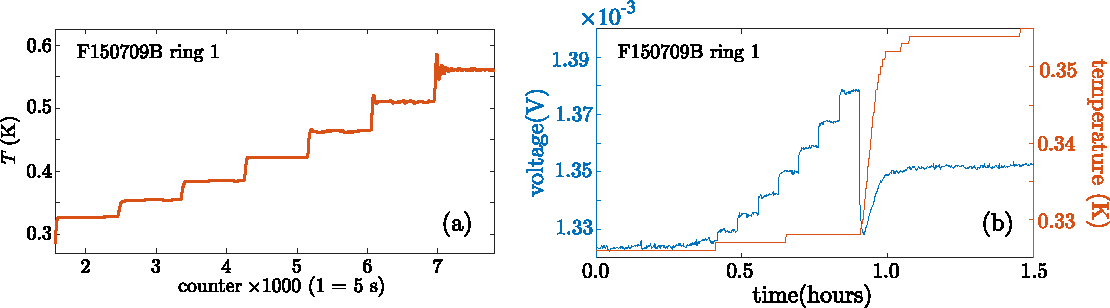
\includegraphics[width=1\textwidth]{figures/temperature_corbino/DCresponseVoltageTempCounter.pdf}
    \caption{Unprocessed measurements of the (a) temperature and (b) voltage response of the system for the same sample and ring. In (a) a set of base temperatures at $P_0 = \SI{0}{\nano\watt}$ was programmed. Figure (b) shows the system response for a set of powers $P_j$ at a specific temperature $T_i$, at  $t \approx \SI{0.9}{\hour}$ an automatic change is produced, the power is again set to zero and a new temperature $T_{i+1}$ established.}
    \label{fig:DCvoltTempCounter}
\end{figure}

A typical temperature measurement it is shown in Fig.~\ref{fig:calT}. Figure \ref{fig:DCvoltTempCounter}(a) shows the system response while changing the base temperature $T_i$. Note that for the lowest temperatures the controller is able to reach easily the set temperature, while once higher settings are placed the system overshoot and a small oscillatory transient must be overcome. This process is time consuming, and the final temperature could change from different runs, this is why we decided to produce the power change measurements once the temperature was reached. This is shown in Fig.~\ref{fig:DCvoltTempCounter}(b), here a set of DC powers $P_j$ was programmed and the temperature and voltage (i.e. current then conductance) was obtained. At time $t \approx \SI{0.9}{\hour}$ the DC heater power is set to zero and a new cold finger temperature established, such change in temperature determines a change in the  conductance minima this is why the voltage changes. After $t = \SI{1.5}{\hour} $ a new set of power changes is made (not shown in this figure). 

Regarding the selected magnetic field position $B_{\nu_0}$ mentioned in item \ref{enum:field}, we could also use the side near a fully quantized filling factor \cite{chickeringPhD}, but the resolution resulted to be lower. Also, when making step \ref{enum:zeroPower} we indicate $P = \SI{0}{\nano\watt}$ but we are actually using the lowest possible configuration of the LIA, $V = \SI{4}{\milli\volt}$. The only way to apply zero power in our setup is to disconnect or short circuit the interconnection box, see Fig.~\textcolor{red}{CITAR FOTO INTERCONEXION BOX}, but this would prevent any automation possibility. We have checked that such minimum voltage (heater power) is below the measurement resolution, even for the thermovoltage measurements, so we can assume it to be zero power.

Finally we obtain a set of calibration curves like the ones shown in Fig. \ref{fig:calT}, for the innermost (ring 1) and outermost (ring 4) rings. Colors correspond to a different powers, each point in this figure is the result of the statistics of 20 measurements once the system stabilizes, after each temperature and power change, see Fig. \ref{fig:DCvoltTempCounter}.  

We want to be able to experimentally determine the temperature gradient on the sample. In order to do so, an interpolation $f(T, G, P)$ is made, from which it is possible to determine a $\Delta t (G) = f^{-1}(G,P)$. To further discuss this approach, say we look at point \textit{a} marked in Fig. \ref{fig:calT} at $T \approx \SI{260}{\milli\kelvin}$ and $P = \SI{277}{\nano\watt}$, we can think of it to be equivalent to point \textit{b} at $P = \SI{0}{\nano\watt}$ and $T \approx \SI{330}{\milli\kelvin}$. So the change in conductance $\Delta G$ is equivalent to a change in temperature $\Delta t$, as shown in that plot.
Because the outer ring saturates its response we can only work this method (in this minima) up to $T = \SI{550}{\milli\kelvin}$. It is important to note that both rings are measured simultaneously.

\begin{figure}
    \centering
    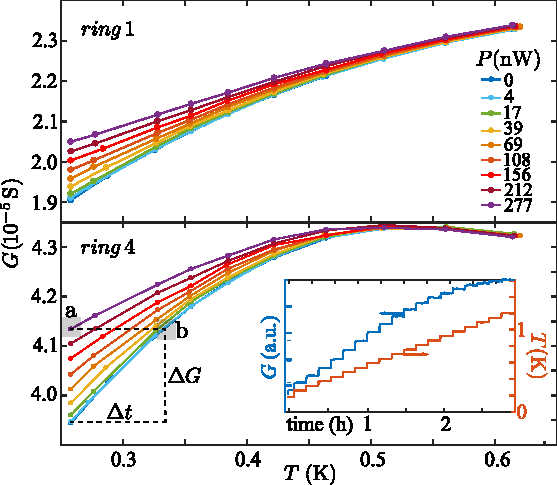
\includegraphics[width=1\textwidth]{figures/temperature_corbino/fig5_calT.pdf}
    \caption{Temperature calibration curves for the innermost (ring 1) and outermost (ring 4) rings. For each temperature and power set, like in Fig. \ref{fig:DCvoltTempCounter}, a point of this plots is obtained. Colors represent different dc heater powers. An interpolation $f(T, G, P)$ is made, from which it is possible to determine a $\Delta t (G) = f^{-1}(G,P)$ for temperatures below $T = \SI{550}{\milli\kelvin}$. It is important to note that both rings are measured simultaneously. \textbf{\textit{Inset:}} Conductance and temperature recorded for $P = \SI{0}{\nano\watt}$.}
    \label{fig:calT}
\end{figure}

From this information we can finally produce a calibration curve like the one shown in Fig. \ref{fig:deltaTpower}. Each point corresponds to the averaged value of the measured temperature difference between rings, i.e. an aproximation of the thermal gradient modulus of the system. The uncertainties include the fitting curves and the statistical error of each point. A deeper understanding and better aproximation of the type B \cite{gum2008} uncertainty should be produced in the future. 

\begin{figure}
    \centering
    \includegraphics[width=0.7\textwidth]{figures/temperature_corbino/deltaTpower_COMSOL.pdf}
    \caption{Temperature calibration curve. Here the temperature gradient measured indirectly between the inner (1) and outer (4) rings are presented. The error bars corresponding to the uncertainty including statistical and interpolated curves. The resulting values of the finite elements modeling of the GaAs crystal for a power of $\SI{277}{\nano\watt}$ is included.}
    \label{fig:deltaTpower}
\end{figure}


In the next section we shall discuss the thermopower response of the system, the model produced from it and the resulting estimated $\Delta T$. 
But we can also estimate the temperature profile using literature values of the thermal conductivity $\kappa$. From the work of Chickering et al.\cite{chickering2013} we deduced a $\kappa_(T = \SI{300}{\milli\kelvin}) \sim \SI{10}{\watt\per\kelvin}$. Using the simulation software finite elements to solve the heat-flow equation given this coefficients a temperature difference of $\SI{2.5}{\milli\kelvin}$ was found between the center and edge of our sample. This results are shown in Fig. \ref{fig:finite elementsDryWet}, there simulations for a wet cryostat (a) and a dry one (b) are shown. The gray area corresponds to the central hole of the Corbino, the ring dimensions are also sketched. Note the deeper slope of the wet system, here the Helium allows a much higher temperature. For further information on this please refer to Appendix \ref{appendixd}. 

\begin{figure}
    \centering
    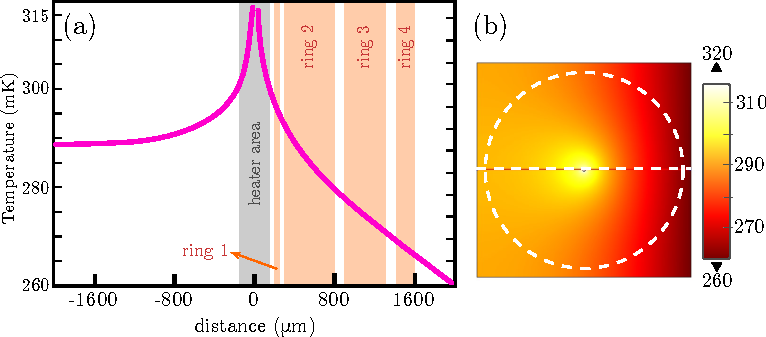
\includegraphics[width=0.7\textwidth]{figures/temperature_corbino/comsol_helium.pdf}
    \caption{Caption}
    \label{fig:finiteElementHe}
\end{figure}

This would lead to a temperature difference across ring 2 of about \SI{1}{\milli\kelvin} that we shall demonstrate to be in good agreement with the value of the thermovoltage theory fit to be discussed. 

\textcolor{violet}{TODO LO ANTERIOR, REVISAR LOS VALORES. TAMBIEN SI LOGRO SACAR BUENOS PLOTS DEL finite elements, INCLUIRLOS ACA Y SEGURAMENTE SERA NECESARIO HACER OTRA SECCION CON ESTO QUE SEA: Heat-flow equation simulation and resulting $\Delta T$}

\begin{figure}
    \centering
    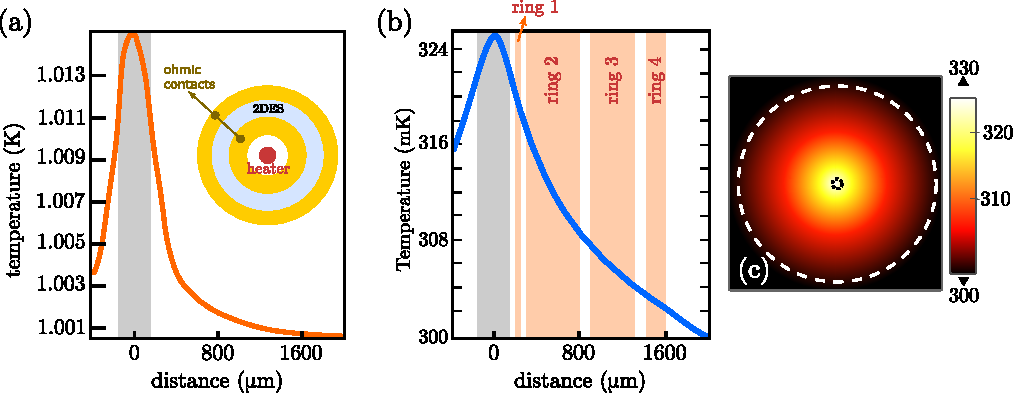
\includegraphics[width=0.9\textwidth]{figures/temperature_corbino/comsol_helium_dry_and_wet.pdf}
    \caption{Temperature profile expected on the samples, produced by a finite elements simulation, original idea by Dr. Werner Dietsche. A central point heating power of P = \SI{277}{\nano\watt} and a standard GaAs thermal conductivity $\kappa = \SI{55}{\watt\per\meter\per\kelvin}$\cite{gaasMTPrus, carlson1965thermal} was used. Sub-figure (a) corresponds to a wet system, while (b) and (c) to a dry one. Notice the faster temperature drop in the case of the wet system. The gray areas indicate sections outside the mesa, where the heater is, wile orange ones to the different Corbino rings. }
    \label{fig:finite elementsDryWet}
\end{figure}


\textcolor{red}{ESTO A OTRO LADO: A note on uncertainty, it must be mentioned that we have not calibrated the LIA under use in this work, they do have a calibration posterior to delivery. They did been verified only against available references.}

\textcolor{red}{OJO CON EL PARRAFO SOBRE EL CERO APLICADO A LA TENSION, ASEGURARSE QUE NO ESTOY MENCIONANDO LA MEDICION DE CALIBRACION DE TEMPERATURA, AHI USABA EFECTIVAMENTE CERO Y UN SMU, SOLO VALE CUANDO HAGO VTP CON EL LOCK IN Y CUANDO HACEMOS CALIBRACION DE TEMPERATURA USANDO }
$f_{\mathrm{in}}= \SI{113}{\hertz}$ unless stated. 





\textcolor{blue}{It is important to note that in our approach the resulting effects and measurements is an average of every direction of the sample, any possible in-homogeneity would be integrated during measurements. But we did not find any signature of such possible effects, like phonon focusing for example.}


\section{sec: Thermovoltage and conductance measurements and modeling}
\label{sec:vtp_g_model}
